\newcolumntype{L}{>{\centering\arraybackslash}m{4.5cm}}

\chapter{Evaluation}
\label{cha:evaluation}
 
\section{Location data characteristics for Berlin area}

\subsection{General overview}

Movement triggered data from mobile devices are spanned across the Germany as shown on \autoref{fig:ger_points}. 
\begin{figure}[!ht]
	\centering
	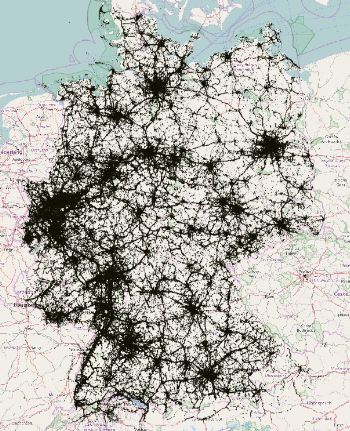
\includegraphics[width=0.3\textwidth]{images/points_germany.png}\\
	\caption{Visualisation of data points location in the geographical map of Germany}
	\label{fig:ger_points}
\end{figure}
\FloatBarrier
It points out, that most of the detected movements from one point to another are mostly gathered on the highways and inside the cities. 
\\
\begin{figure}[!ht]
	\centering
	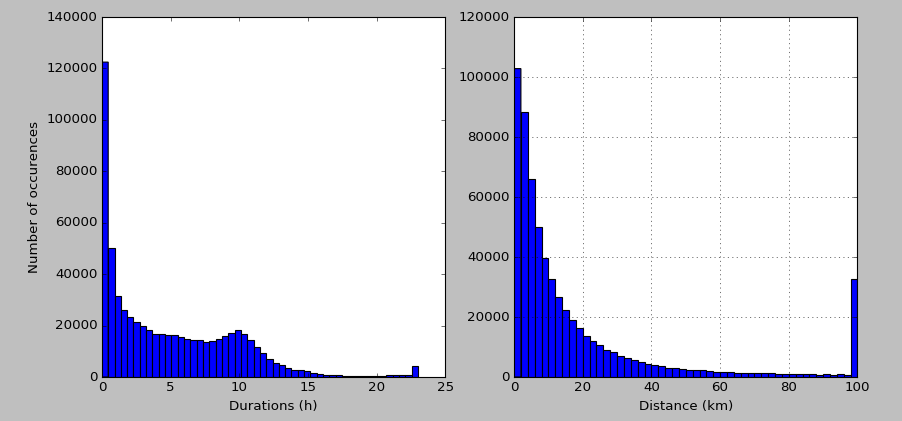
\includegraphics[width=0.9\textwidth]{images/germany_stats.png}\\
	\caption{Histograms of durations and distances between consecutive points under and cumulatively over 100 km for the area of Germany}
	\label{fig:ger_stats}
\end{figure}
\FloatBarrier
The given data batch has been gathered in the interval of 24h starting from 3am in the morning German time. It consists of over 675000 data points, belonging to 47300 unique mobile devices. \autoref{fig:ger_stats} shows, that for unique mobile devices, the durations between consecutive points in time are most frequent within 30 minutes and most of the data is in the interval 1-10h. Regarding distances, consecutive points are most frequent below 2 km and most data is in the interval 0-10km. Big chunk of distances is also over 100km.     
\\
\begin{figure}[!ht]
	\centering
	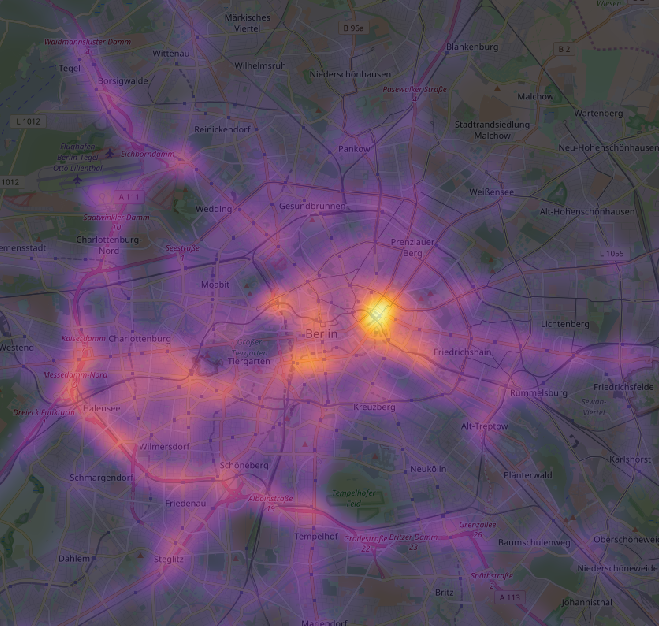
\includegraphics[width=0.9\textwidth]{images/points_berlin_heatmap.png}\\
	\caption{Heatmap of data point densities within the area of Berlin}
	\label{fig:ber_heat}
\end{figure}
\FloatBarrier
\autoref{fig:ber_heat} shows the heatmap of data points for Berlin area. We can see that most of the movements detected are on major train/tram/metro stations, highways and major living areas. 

\subsection{Data analysis}
\label{cha:dataanaly}

Statistics performed using tool written in Python (https://github.com/mrow4a/macroscopic-movements-algorithm-prototypes) shows, that for users at least once visiting Berlin, had in average 17 points gathered because of their movements in the period of 24h, harmonic mean of 4 points and maximum 100 of points.
\\
\begin{figure}[!ht]
	\centering
	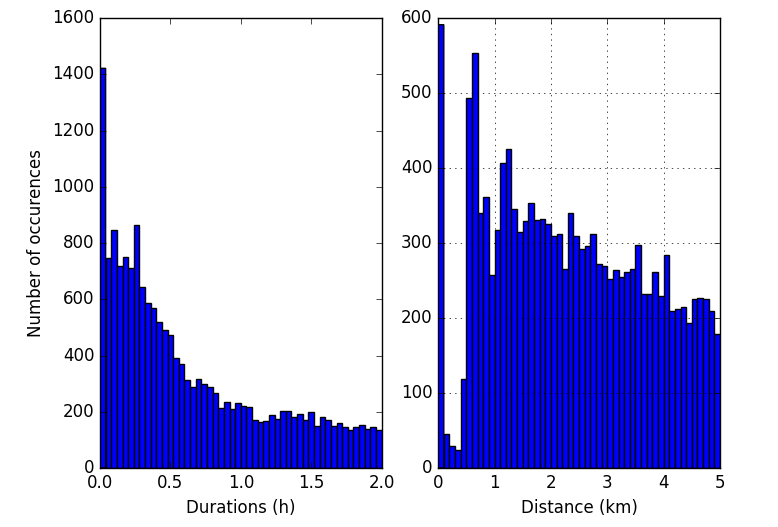
\includegraphics[width=0.6\textwidth]{images/berlin_stats_intro.png}\\
	\caption{Histograms of durations and distances between consecutive points under 5 km and under durations of 2h for the area of Berlin}
	\label{fig:ber_stats}
\end{figure}
\FloatBarrier
Furthermore, majority of durations between points is within interval of 30 minutes. For distances between points, there is significant "jump" at 500-1000m and 1100-1500m, which might mean that at these intervals, continuous points been gathered, and distances over that values might be discontinuous (ref. \autoref{fig:movement_update} ). It is due to the fact that these distance intervals are most frequent and that might suggest that this is an average "update" distance for the moving mobile devices, as described in \autoref{cha:introduction_methodo}. Less frequent values might suggest that updates were obtained with lower accuracy (e.g. by presence inside the building, metro line or simply mobile device lag in obtaining its location) and are result of discontinuity between consecutive updates.
\begin{figure}[!ht]
	\centering
	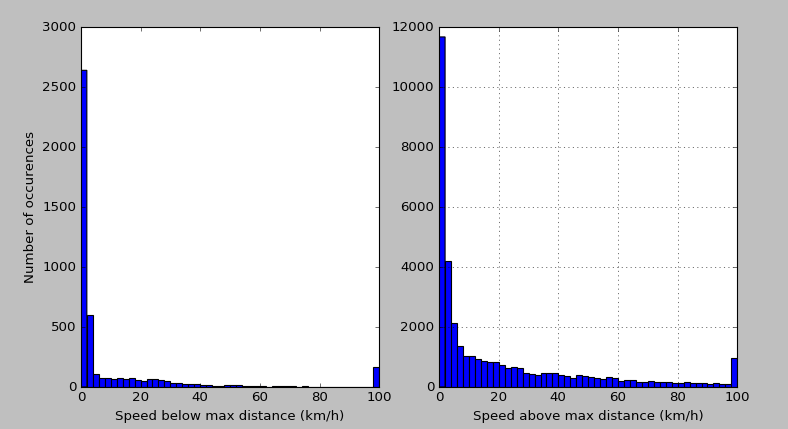
\includegraphics[width=0.6\textwidth]{images/berlin_speeds_distances.png}\\
	\caption{Histogram of speed between points with corresponding distance above or below 1.5 km}
	\label{fig:ber_sp_dis}
\end{figure}
\FloatBarrier
\autoref{fig:ber_sp_dis} shows that considering the registered distances within range of 1500m, the wast majority of points are between 0-2 km/h, and also significant interval at 2-6 km/h. The rest of the values is sparse distributed in interval 6-100+ km/h. In case of registered point above range of 1500m, we observe that indeed most frequent occurrence is at interval of 0-4 km/h, however most are sparse distributed above 4 km/h, with most points being in interval of 4-20 km/h. 

\section{Pre-filtering of anomalies}
\label{cha:prefilter}
\autoref{fig:ber_stats} shows that there is a fraction of points which duration or distance rapidly changed, thus resulting in very high speeds between the points. Points having speeds above 300 km/h and distances above 100km can be considered as flights, however the ones below 100km are anomalies. \autoref{fig:anom1} shows that number of flights in Germany has not been significant (around 100) compared to number of speed anomalies (over 25000).
\\\\
Furthermore, due to the methodology of obtaining points (movement triggered), there are some minimum distances and durations at which points can be collected, and values not matching stop or travel expectation according to gathered statistics, have to be filtered and considered as duplicates. 

\begin{figure}[!ht]
	\centering
	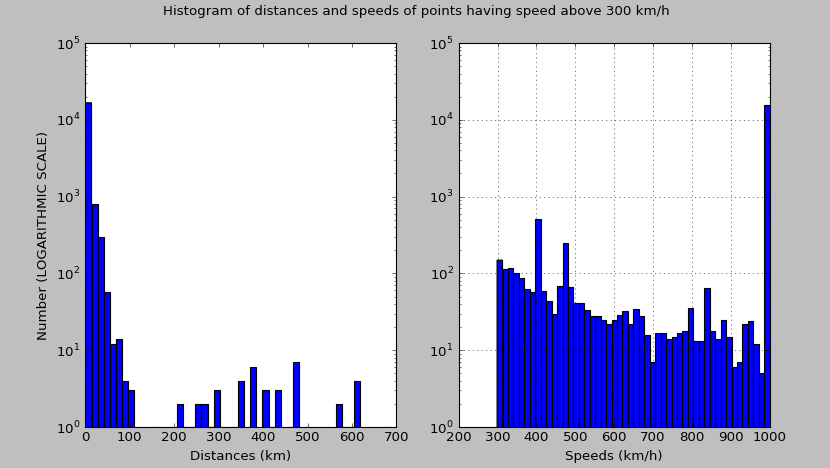
\includegraphics[width=0.6\textwidth]{images/anom1.png}\\
	\caption{ Speeds and distances histogram of points having speeds above certain threshold }
	\label{fig:anom1}
\end{figure}
\FloatBarrier

Thus, the following predicates for filtered values have been set:
\begin{description}
	\item[Jumps] Points with speed over 83 m/s [300 km/h] and at the same time distance below 100 km/h
	\item[Duplicates] Points with distance below 100m and at the same time duration below 100s
\end{description}

\section{Evaluation of stop detection algorithms}

\subsection{Mobility Index approach}

Mobility Index analysis is performed in order to detect single movements or series of movements to be classified as stop or slow movement over the restricted area. 
\\\\
By the nature of mobility index, more values in the window, higher the mobility index is. Thus, if only one value is in the window, one can apply "stop duration" threshold, however if windows contains more values, we require higher threshold to be able to fit sum of inverses of the movements. 
\\\\
As an example, having window of 20 minutes and threshold of 1/(10 minutes), if we fit into window single point with duration of 15 minutes, this value will be classified as a stop. However, if we obtain 2 values, 5 and 10 minutes respectively (1/5 + 1/10), our threshold requires to be higher in order to include slow movements in the window and classify this 2 values as stop in restricted area.

\begin{figure}[!ht]
	\centering
	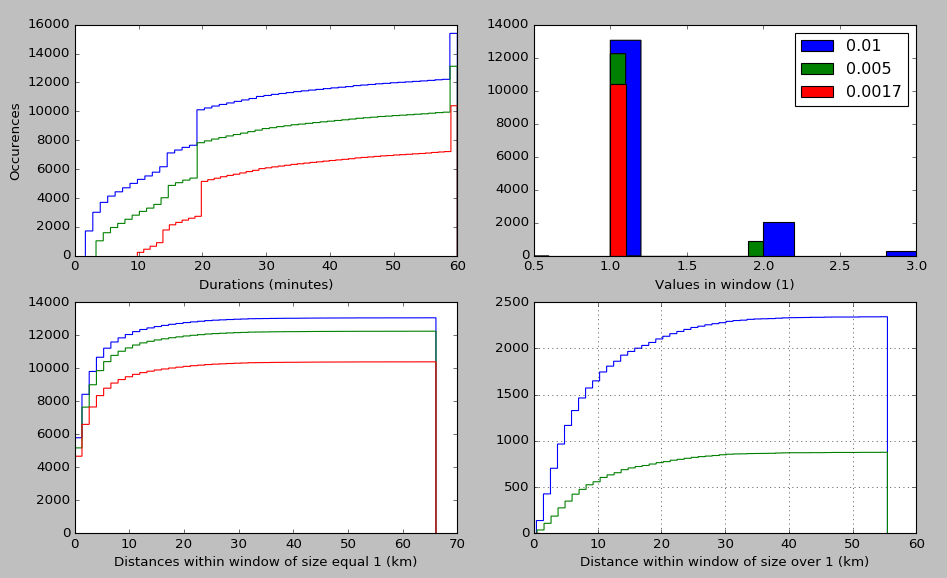
\includegraphics[width=0.95\textwidth]{images/mob_index_analy1.png}\\
	\caption{ Analysis of detected stops for varying MobilityIndexThreshold for time window of 20 minutes. Cumulative distribution of inverted mobility index (top left). Histogram of window sizes (top right). Cumulative distributions of total distances between points in the window of size 1 (bottom left) and above 1 (bottom right). }
	\label{fig:mob_index_analy1}
\end{figure}
\FloatBarrier

\autoref{fig:mob_index_analy1} shows the analysis of the stops detected using mobility index, using sliding time window approach.
\\\\
Cumulative distribution of inverted mobility index (top left) shows that for window of 20 minutes, increasing MobilityIndexThreshold from 0.0017 (1/10 minutes) to 0.01 (1/2minutes), sum of inversions of durations (MobilityIndex) for points within the window, increases total number of stops from 10000 to 15000, where the increase (5000 points) is caused by points in the range 2-10 minutes, which is expected result increasing the threshold. The rapid jump at 20 minutes is caused by the fact that at that threshold some inverted mobility indexes were result of summing window of more then one value. 
\\\\
Histogram of sizes of the window (number of points within a 20 minutes window - top right) shows, that with parameter 0.0017, all the points are contained within the windows having size of 1 point. Increasing the threshold to 0.005 (1/4 minutes), it resulted in 95 percent of points being in windows of size 1 and 5 percent in windows of size 2 (2 points in the window - restricted area of stop). Doubling the threshold to 0.01 resulted in 75 percent being in single value window, and 25 percent in over 2 points per window. 
\\\\
The graphs in the bottom of \autoref{fig:mob_index_analy1} show what are the distances covered in the windows having 1 or more points. It occurs, that in case of 1 point in the window (which means that this point is a stop), distances between points range from 0 to 60km, and this is expected. However, in case of 2 or more points per window (thus stops within a restricted area bound by points), it occurs that only small fraction of values has total distance covered less then 2km, and major fraction of points represent long distance covered. 
\\\\
The above analysis shows, that mobility index cannot be effectively used to detect group of points which might be considered as a stop and only very small fraction of windows having more points then 1 is considered as a stop within a small restricted area. The rest is spanned across bigger distances. Thus, small values of mobility index window and threshold might start detecting trips over longer distance as a stop and providing erroneous results. 
  
\begin{figure}[!ht]
	\centering
	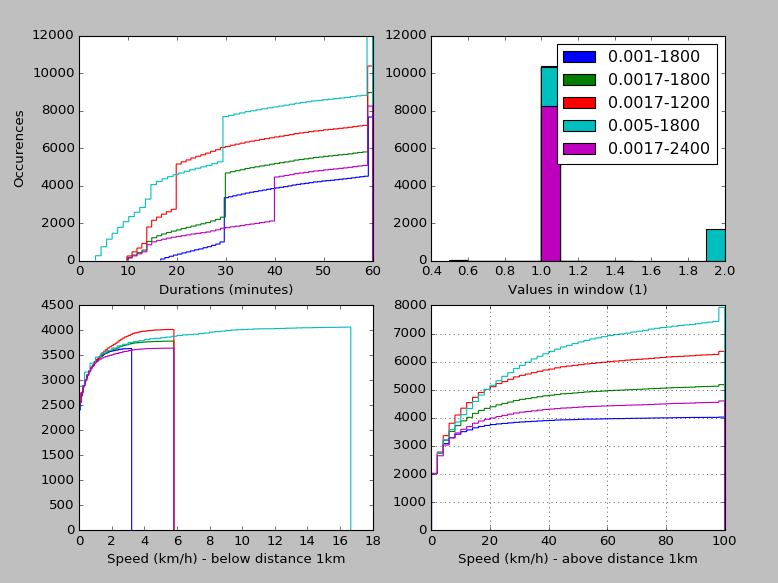
\includegraphics[width=0.95\textwidth]{images/mob_index_analy2.png}\\
	\caption{ Analysis of detected stops for varying MobilityIndexThreshold-MobilityIndexWindow(seconds), correspondingly as in the label of measurement. Cumulative distribution of duration for detected stops (top left). Histogram of window sizes (top right). Cumulative distributions of speed between point for distance below 1km (bottom left) and above 1km (bottom right). }
	\label{fig:mob_index_analy2}
\end{figure}
\FloatBarrier 
 
\autoref{fig:mob_index_analy2} shows the analysis of the stops detected using mobility index threshold, using sliding time window approach, however in this case it is used to identify mobility of a user considering only last recorded point in the window to decide if the movement can be a stop considering its past mobility.
\\\\
This approach tries to tackle the problem discussed in \autoref{cha:stopdet_bh}, where it has been said that over longer distances e.g. 2-10 km between recorded points, detection using speed is difficult since stop for a short time and movement with high speed will produce very high average speed in that time period. 
\\\\
\autoref{fig:mob_index_analy2} gives cumulative histograms considering different pair of parameters (MobilityIndexThreshold-MobilityIndexWindow) considered in producing stop locations. Cumulative distribution of duration at detected stops (top left) shows that considering the same MobilityIndexThreshold (0.0017-1200s, 0.0017-1800s, 0.0017-2400s) and increasing MobilityIndexWindow, causes less stops to be detected and higher average duration between points detected. Considering the same MobilityIndexWindow (0.001-1800s, 0.0017-1800s, 0.005-1800s) and increasing MobilityIndexThreshold, number of stops increases, and this increase is bound only to values below MobilityIndexWindow threshold. High MobilityIndexThreshold produces more stops with shorter duration of stop. 
\\\\
Cumulative distribution of speed for detected points show that algorithm with all tested parameters has been able to identify correctly stops over distance less then 1km and with very small speeds (long stay duration at the point). However, MobilityIndexThreshold or decreasing MobilityIndexWindow cause that average speed of detected points had higher speed over distances > 1km and these were not able to filter trips over long distances correctly. For thresholds 0.001-1800s, 0.0017-1800s and 0.0017-2400s higher speeds are being filtered and only longer stays are left, and the difference between performance of these parameters is a trade-off between an accuracy and number of detected stops. 
\\\\
Histogram of values in the window (top right) also confirms, that for 0.001-1800s, 0.0017-1800s and 0.0017-2400s thresholds, detected stops had window of 1 value, thus none of the windows having 2 or more values were not qualified for being a stop and thus being filtered out as high mobility trip. This behavior of algorithm allows to identify stays with simple duration threshold and at the same time filter out all multi-point trips using mobility index window. 

\subsection{Human Mobility approach for long/short distances}

Speed/Distance analysis is performed in order to detect single movements as stop or slow movement. If the average speed between the points is below the certain threshold, it is assumed to be a stop. 
 
\begin{figure}[!ht]
	\centering
	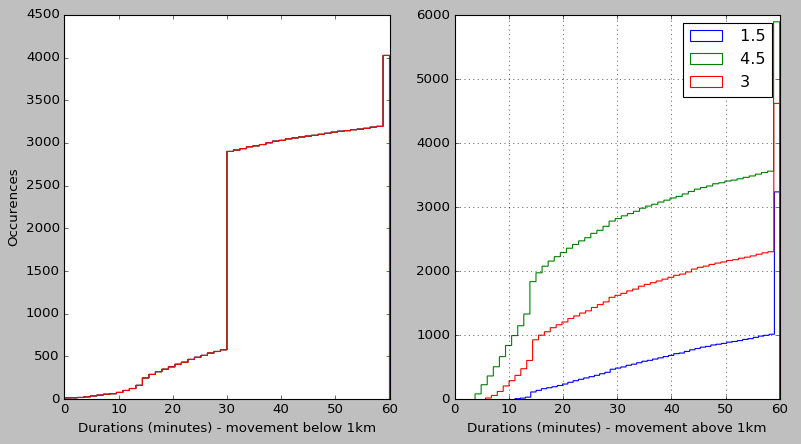
\includegraphics[width=0.95\textwidth]{images/speed_dist_analy1.png}\\
	\caption{ Speed/Distance detection with StopCertaintyMaxDistance, StopCertaintyMaxSpeed and TravelCertaintyMinSpeed thresholds. Cumulative distribution of duration for detected stops below and above distance StopCertaintyMaxDistance of 1km for different  TravelCertaintyMinSpeed thresholds. }
	\label{fig:speed_dist_analy1}
\end{figure}
\FloatBarrier 

\autoref{fig:speed_dist_analy1} shows analysis of detected stops having TravelCertaintyMinSpeed varying and StopCertaintyMaxSpeed fixed. Increasing the speed threshold for points above 1km, we observe that number of points in interval 15 to 60+ minutes stays fixed for all parameters, however increasing threshold increases number of stops detected in interval 5-15 minutes diracticaly. It means, that with these thresholds, much more movements which has very low duration over the distance are classified as a stop and identification might be erroneous to mislead long distance trip with a stop. 
\\\\
Furthermore, having TravelCertaintyMinSpeed threshold of 1.5 m/s, we can see that speed threshold correctly identifies the stops, however the number of detected stops in the movements above 1km compared to mobility index approach is low (\autoref{fig:mob_index_analy2})
\\\\
On the other hand, for distances below 1km, speed detection has not only been able to identify longer stays at location, but also a short distance, very slow movements over the area, successfully. 

\subsection{Conclusions}

\begin{table}[h!]
	\centering
	\caption{Comparison of two analyzed stop detection algorithms for proactive localization}
	\label{tab:alg_comp_table}
	\begin{tabular}{|L|L|L|}\hline
		\textbf{Case} & \textbf{Mobility Index} & \textbf{Speed/Distance} 
		\\\hline
		Slow movements over small area or distance & Possible, but adjusted parameters will cause results to be erroneous for different detections & Very good
		\\\hline
		Stays at short distance & Good, but only for longer stays & Very good  
		\\\hline
		Stays at long distance & Very good, but only in case of adjusted parameters which might be erroneous at short distances & Possible, but might be erroneous and stops maybe mislead with travel due to high speed averages in these cases
		\\\hline
	\end{tabular}
\end{table}
\FloatBarrier 

\autoref{tab:alg_comp_table} shows comparison of two approaches to stop detection. It occurs, that for short distances it is more efficient to use speed/distance algorithm to be able not only capture longer stays at short distance, but also very slow movements in the limited area. For longer distances it is preferable to use mobility index to be able distinguishing travels from stops better using mobility index, which preserves mobility history for the certain past time window. MobilityIndexWindow becomes a duration threshold at which mobility window with multiple points is being accepted, and MobilityIndexThreshold is defining at which multiple points or single point cannot be classified as a stop and be a series of movements/movement. 

\section{Clustering algorithm}

In this section we will describe how we evaluated our dbscan algorithm and the choice of the \textit{epsilon} and \textit{minimum points per cluster} parameter.

\subsection{DBSCAN}

We visualised our results in QGIS, a powerful graph visualisation tool. Running the dbscan with different parameters resulted in different cluster sizes and number of clusters. We started off with the target area of Berlin. The \textit{epsilon} parameter (radius of the cluster) was chosen by looking at the graininess (accuracy) of our given data set. The accuracy between points was 110 meters, this distance is refered to as \textit{accuracy distance}.
We took Alexanderplatz in Berlin as an example cluster (a popular train stop area in Berlin). We interpret one cluster as being one stop point of interest, and for this application want Alexanderplatz to be represented as one cluster. Setting the \textit{epsilon} parameter to the \textit{accuracy distance},  110 meters, gave us good looking clusters whilst higher value of the parameter resulted in clusters being unnaturally large and distance below the \textit{accuracy distance} resulted in only single-point clusters (points are stacked at the same location). Note that the \textit{minPts}, minimum points per cluster, parameter is not taken into \textit{consideration} here (it is set arbitary and only determines the number of clusters, while we here are interested in the \textit{size} of the clusters). See figures below.

\begin{figure}[!ht]
	\centering
	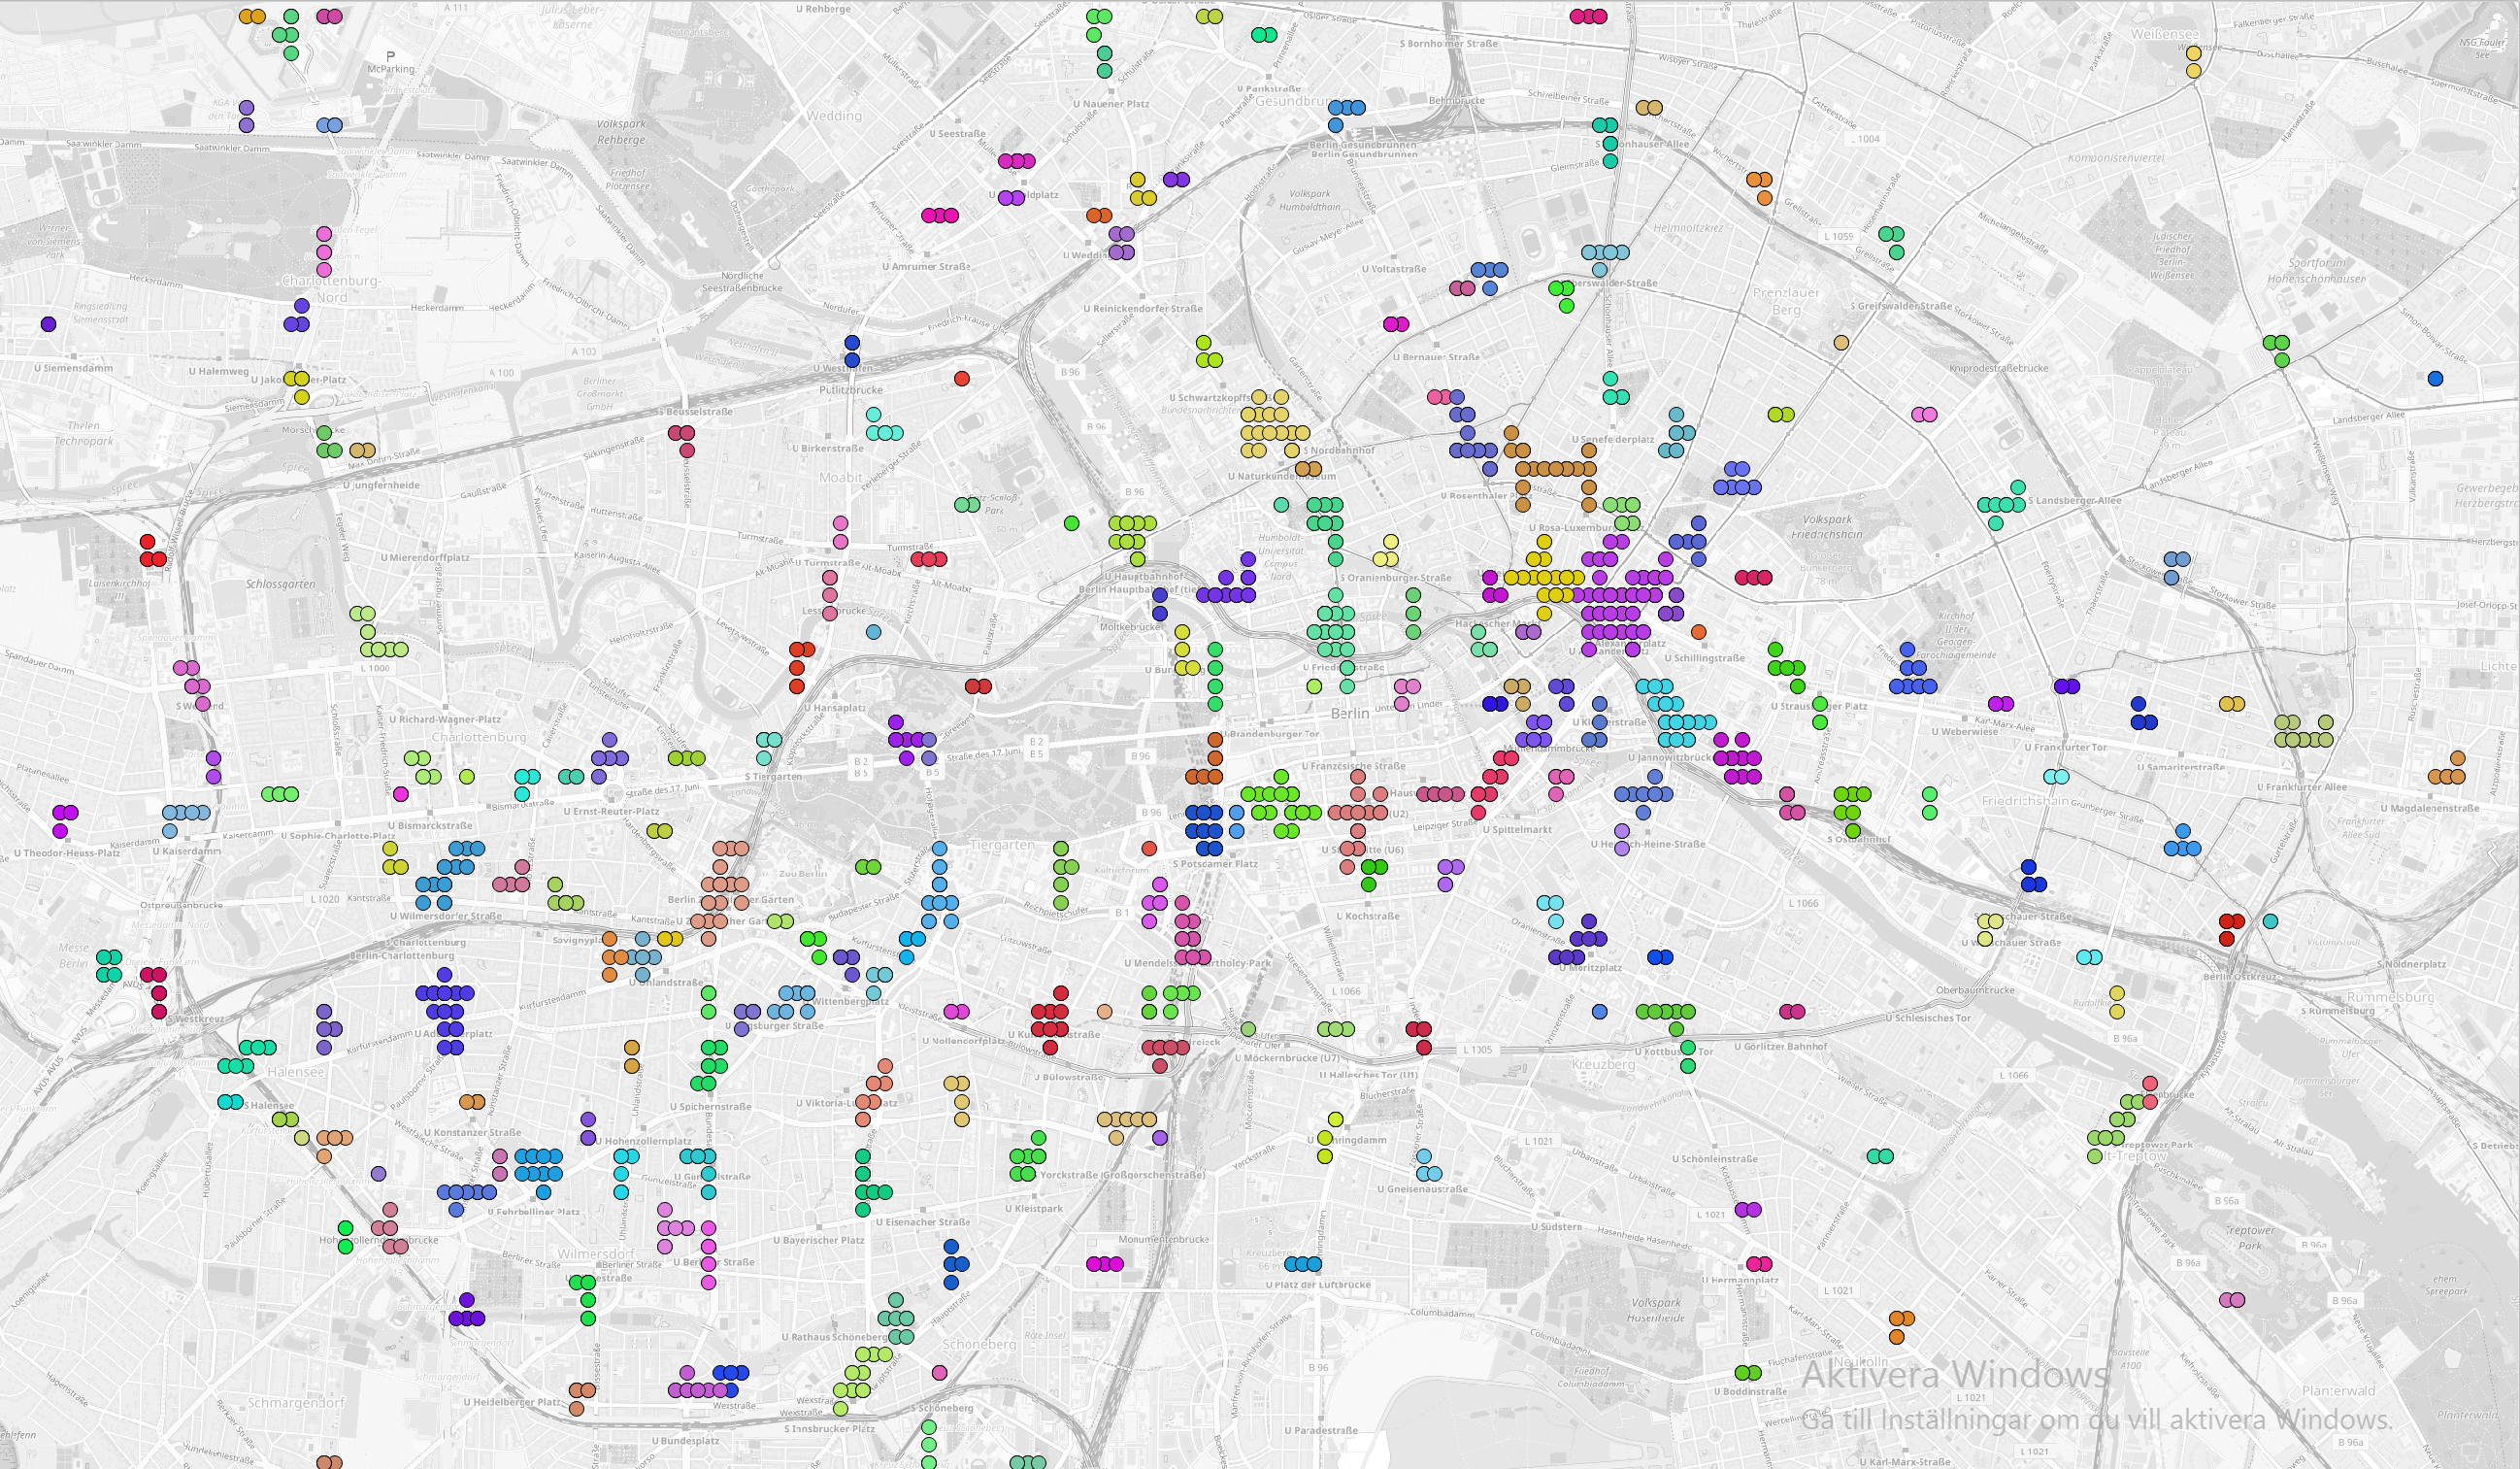
\includegraphics[width=1\textwidth]{images/0,001_5_gray.png}\\
	\caption{ Clusters with good parameters \textit{epsilon} = 110 meter, \textit{minPts} = 5. Alexanderplatz (pink) has 85 data points in it.  }
	\label{fig:0.001_5_gray}
\end{figure}

\begin{figure}[!ht]
	\centering
	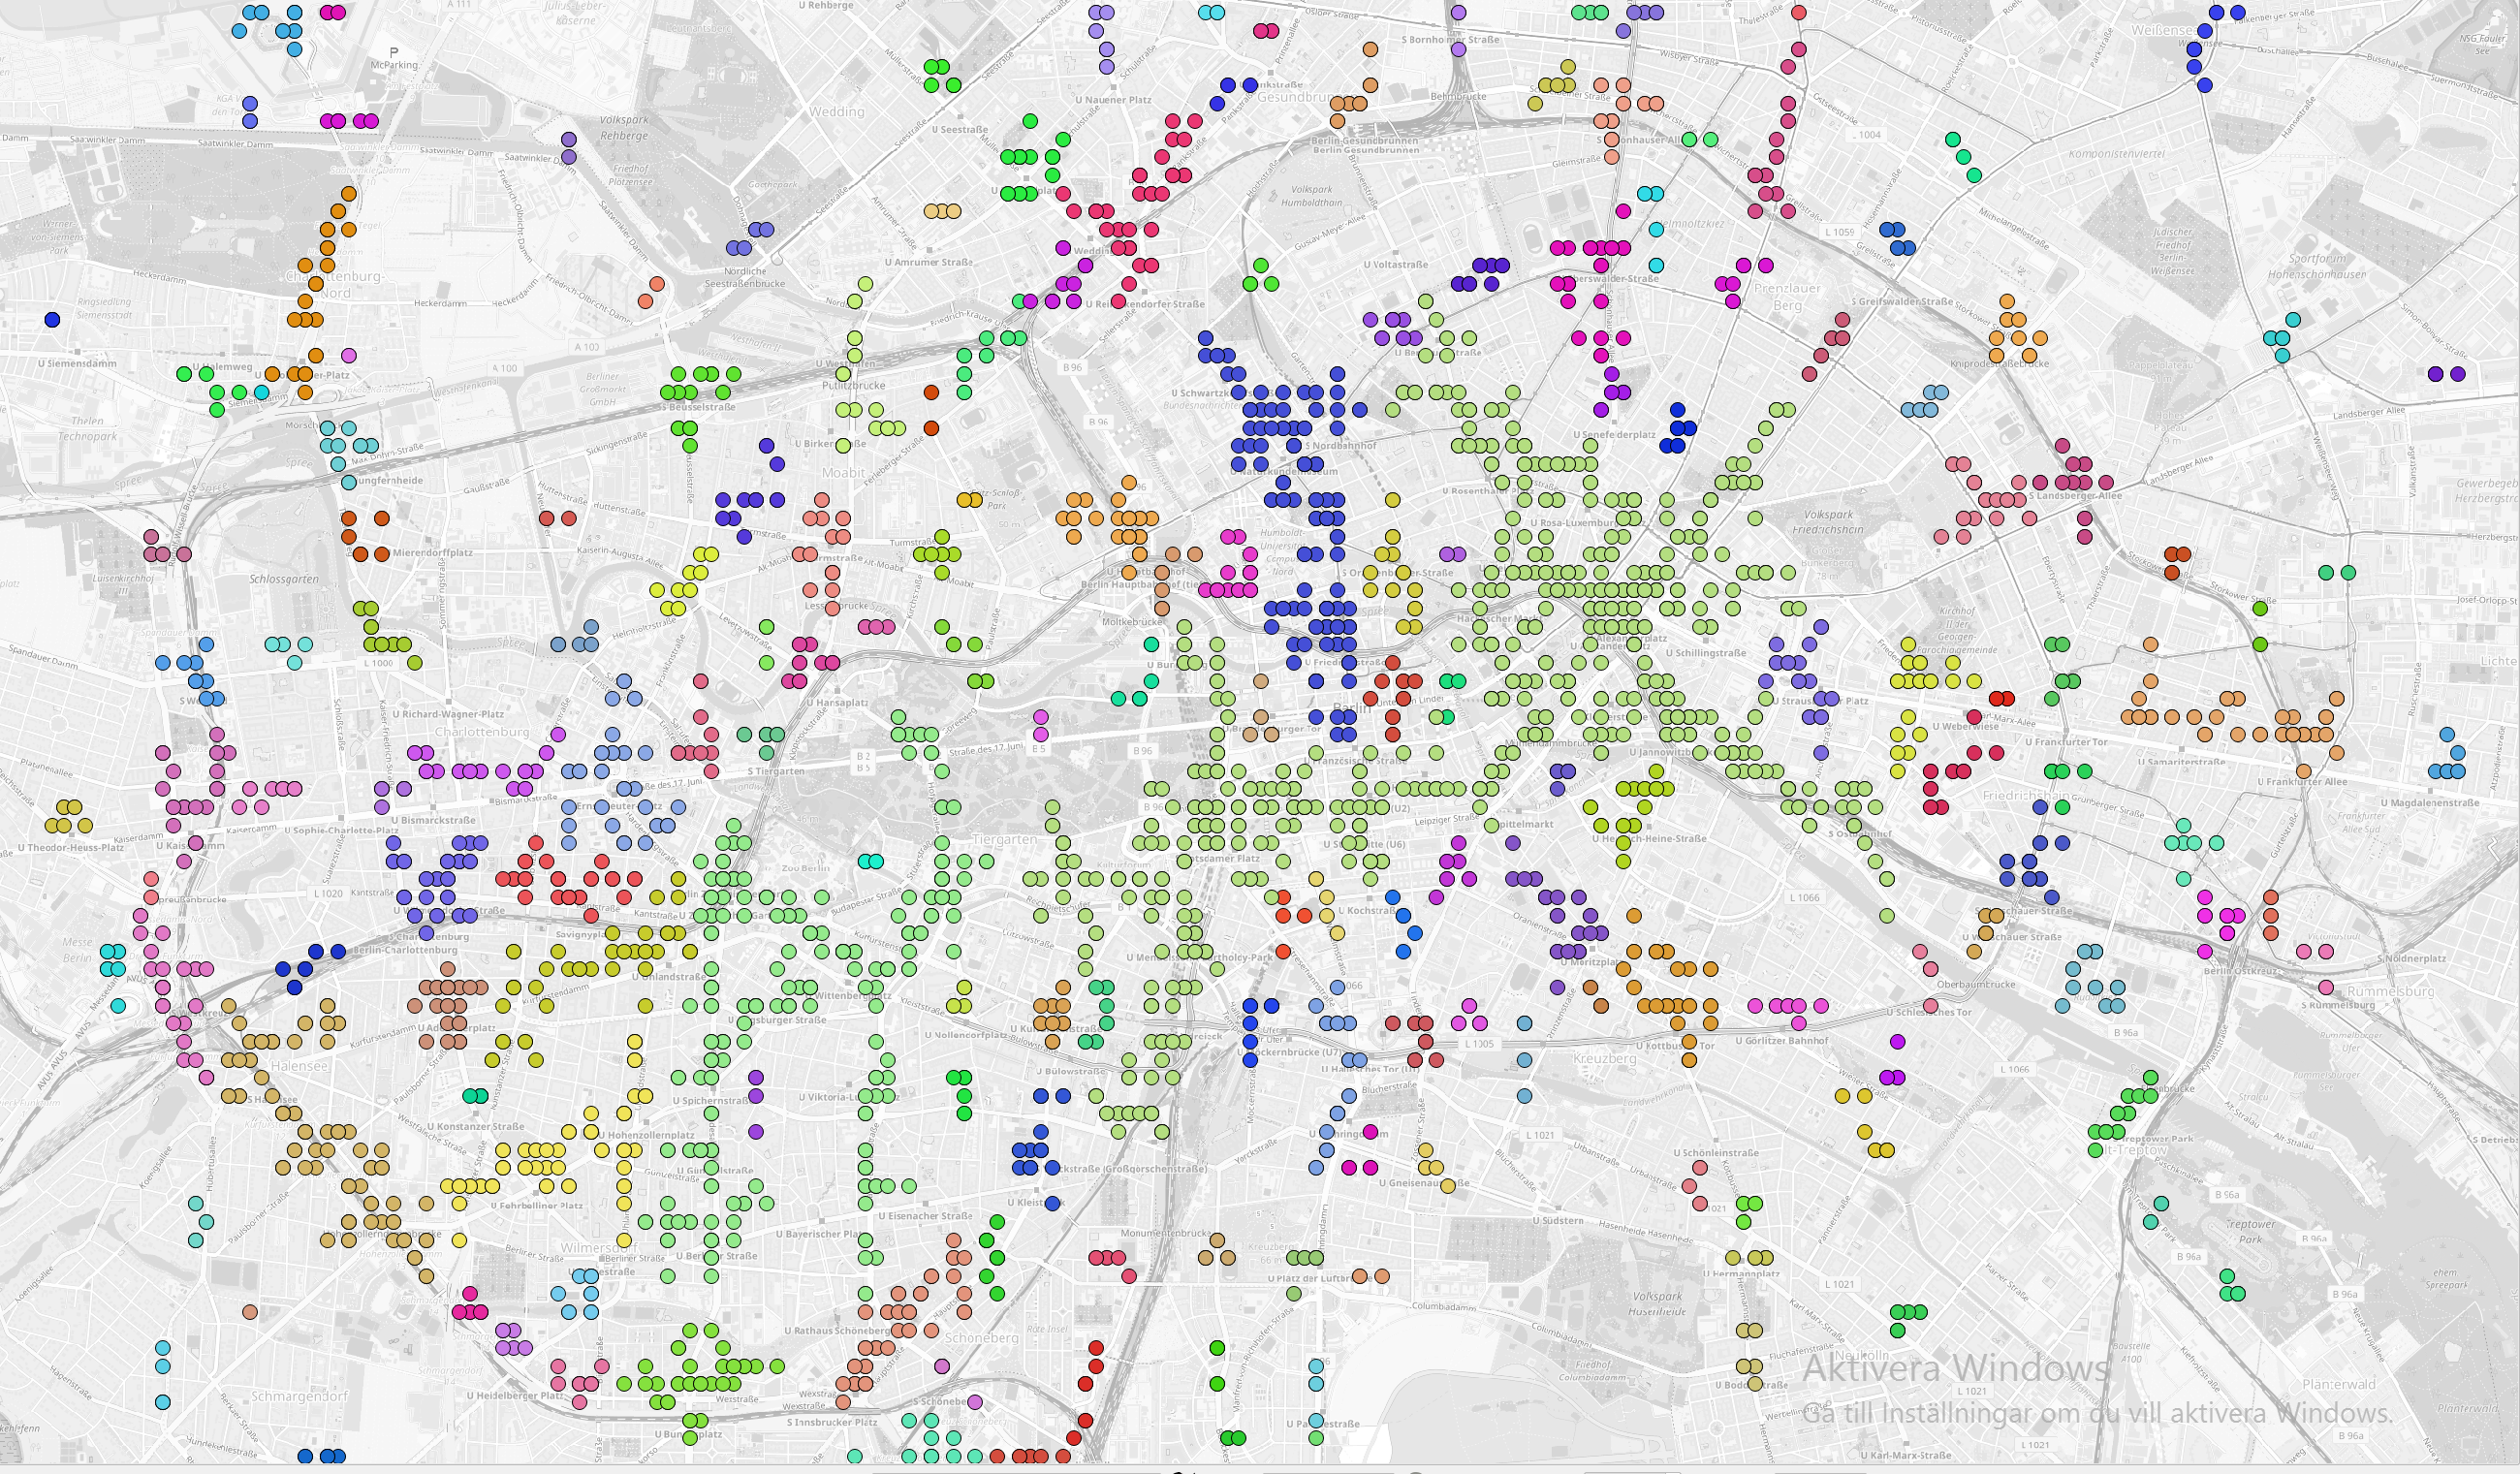
\includegraphics[width=1\textwidth]{images/0,002_5_gray.png}\\
	\caption{ Example of a clusters with bad parameters, here \textit{epsilon} = 220 meter is too large, \textit{minPts} = 5. "Alexanderplatz" (light green) has 748 data points in it and stretches over the whole centre (Mitte) of Berlin. }
	\label{fig:002_5_gray}
\end{figure}